\documentclass[12pt]{article} 
\usepackage[francais]{babel}
\usepackage[T1]{fontenc}
\usepackage[utf8]{inputenc}
\usepackage{eurosym}
\usepackage{array}
\usepackage{graphicx}
\usepackage{fancyhdr}
\usepackage{verbatim}
\usepackage{enumerate}

\pagestyle{fancy}
\fancyhf{}
\rhead{Issidi}
\lhead{Rapport de 2\ieme{} soutenance}
\rfoot{Page \thepage}


\title{Rapport de 2\ieme{} soutenance\\
		Issidi\\
		Debil.OS();}
\author{Jérémy \bsc{Beuvry}\\
		Julien \bsc{Boulicaut}\\
		Clément \bsc{Finck}\\
		Sébastien \bsc{Fleury}}

\begin{document}
\maketitle
\centerline{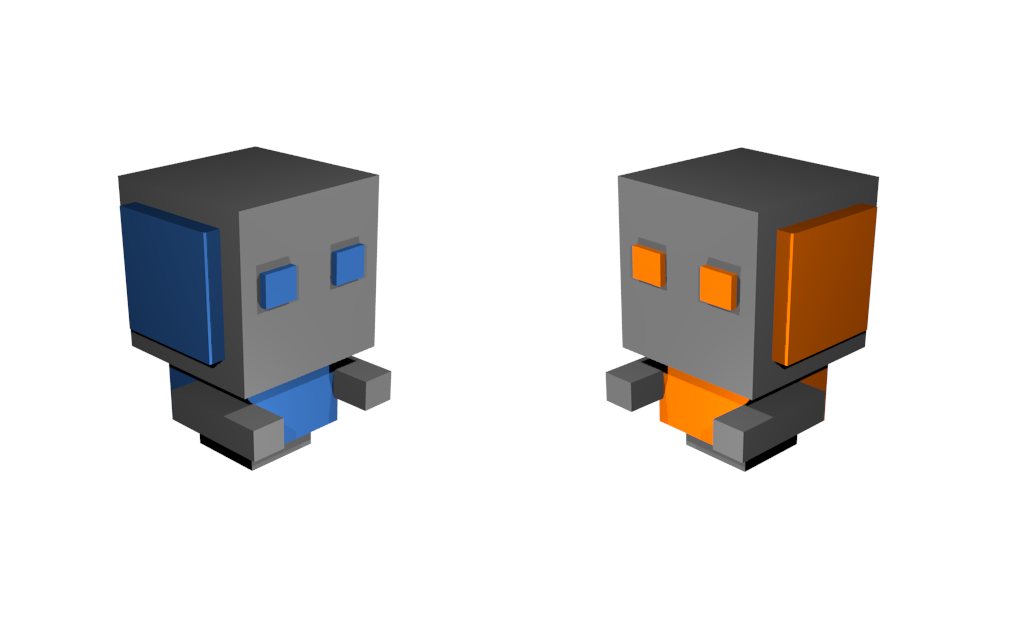
\includegraphics[scale=0.4]{rf.png}}
\newpage
\tableofcontents
\newpage

\section{Introduction}
Notre groupe, les ''Debil.OS();'' est fier de vous présenter son second rapport de soutenance du projet Issidi.
\newline\newline Ce projet prend la forme d'un jeu de tir à la troisième personne dans un univers post apocalyptique.  Les principal mécaniques du gameplay et l'univers sont rappeler 

\centerline{
\includegraphics[scale=0.2]{latex_sa_pue.png}}
\centerline{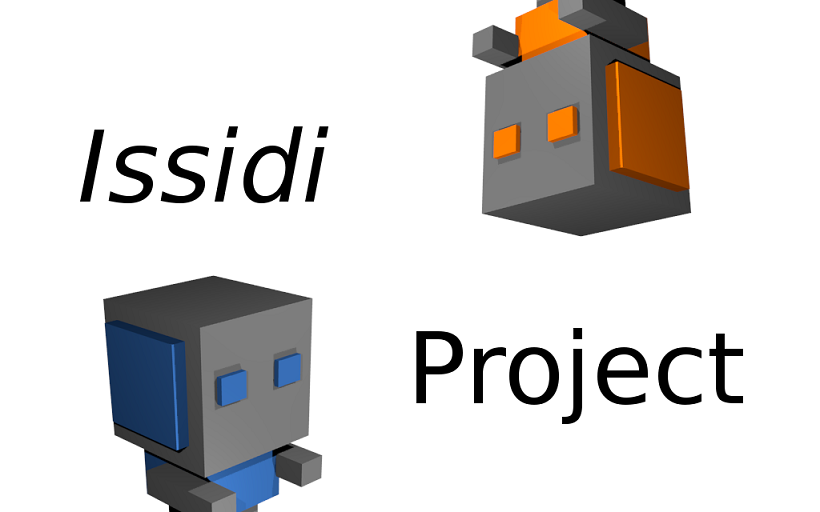
\includegraphics[scale=0.5]{styler.png}}


\newpage\section{Rappel du cahier des charges}

\subsection{Mécanique de jeu}
\centerline{
\includegraphics[scale=0.2]{latex_sa_pue.png}}

 Issidi est un jeu de tir à la troisième personne(aussi appelé \emph{Third Person Shooter}),
qui sera créé avec le moteur de jeu Unity3d, édition personnelle.

Pour les déplacement en plus de ceux classique vous pourrez également esquiver à l'aide de petit saut rapide vers 
l'avant ou encore utiliser des doubles sauts qui permettront aussi d'atteindre certaines zones qui auraient
 été inaccessibles sinon.

Plusieurs armes seront disponibles pour varier le gameplay et permettre à tous les types de joueurs de prendre
 un maximum de plaisir. Que vous adorez tout faire exploser avec une lance rocket, ou un rythme plus rapide avec 
un fusil d'assaut, même les fans de corps à corps pourront même s'essayer à la vivisection laser sur robots. 
ainsi que différentes cartes.

Le mode multijoueurs mettra en scène les batailles sanglantes entre pillards de ressources dont un seul 
sortira vainqueur, ou pas !


\subsection{Physique}
Cette section sera dédiée à la gestion des interactions des différents éléments avec la gravité.
Ainsi que la gestion de tous les types de collisions: joueur/terrain,projectile/joueur, projectile/terrain ( pour à terme, permettre d'avoir un
environnement partiellement destructible). Parmi les interactions on notera en particulier la possibilité de marcher sur 
les murs et le plafond, via une rotation du vecteur gravité, qui constituera l'une des principales mécaniques du jeu.

\subsection{Arme}
Un robot sans défense n'a aucun intérêt s'il ne possède rien lui permettant d'occire ses ennemis, 
il doit donc disposer d'un arsenal suffisant. Il sera donc nécessaire de créer plusieurs armes
afin d'ajouter une profondeur au gameplay.


\subsection{Interface}
Afin de rendre le jeu plus convivial, celui-ci doit posséder 
une interface composée de plusieurs menus. Celle-ci 
permettra notamment de naviguer dans les options du jeu, de
 lancer une partie en mode solo, ainsi que de choisir les
 paramètres des parties du mode multijoueur.

\newpage\subsection{Site Web}
Le site web nous permettra de montrer l'avancement de notre projet.Il contiendra une description du projet, des images de celui-ci, ainsi
que des liens permettant d'avoir un accès rapide aux sources du projet.

\section{Répartition des tâches}

\begin{tabular}{|c|c|c|c|c|}
\hline
			&	Jérémy		&	Julien		&	Clément		&	Sébastien	\\ \hline
Site Web	&				& $\bigotimes$	& 				& $\bigcirc$	\\ \hline
Physique	&				&				& $\bigcirc$	& $\bigotimes$	\\ \hline
Multijoueur	& $\bigotimes$	& $\bigcirc$	&				& 				\\ \hline
Animation	&				& $\bigotimes$	& $\bigcirc$	&				\\ \hline
IA			& 				& $\bigotimes$	& $\bigotimes$	&				\\ \hline
Particules	& $\bigcirc$	& 				&				& $\bigotimes$	\\ \hline
Personnage	& $\bigotimes$	&				& 				& $\bigcirc$	\\ \hline
Arme		& $\bigcirc$	&				&				& $\bigotimes$	\\ \hline
Son			&				& $\bigcirc$	& $\bigotimes$	&				\\ \hline
Modèles		& $\bigotimes$	&				& $\bigotimes$	&				\\ \hline
Interfaces	& 				& $\bigcirc$	& $\bigotimes$	&				\\ \hline
\end{tabular}

Légende:\\
$\bigotimes$ : s'occupe de\\
$\bigcirc$ : aide

\section{Éléments déja effectués}
\subsection{Interface}
\begin{itemize}
\item[+] Ajout du menu principal
\item[+] Ajout d'un menu pause
\item[+] création de la barre de vie
\end{itemize}

\subsection{Physique}
\begin{itemize}
\item[+] Ajout d'une boite de collision pour le personnage, afin de lui permettre d'évoluer dans le monde
\item[+] Modification de la gravité en fonction de son axe
\item[+] Changement de l'axe du personnage lors de l'appui sur \emph{E}.
\end{itemize}

\subsection{Particules}
\begin{itemize}
\item[+] Les balles sont suivit de particules, représentant la traînée.
\end{itemize}

\subsection{Personnage}
\begin{itemize}
\item[+] Possibilité de se déplacer
\item[+] Échange possible de son axe de mouvement
\item[+] Le personnage peut dasher (accélérer brutalement), impossibilité de changer de direction lors du dash
\item[+] Double sauts possible
\item[+] Caméra à la 3\ieme{} personne
\item[+] Possibilité de se déplacer
\end{itemize}


\subsection{Arme}
\begin{itemize}
\item[+] lance-flamme
\item[+] lance-rocket
\end{itemize}


\subsubsection{Créations des modèles}
\begin{itemize}
\item[+] Personnages
\item[+] Armes variées
\item[+] Point de respawn
\item[+] Tourelles
\item[+] Araignée suicidaire
\item[+] Map prédécoupé
\end{itemize}

\section{Planning de la 2\ieme{} soutenance}
\begin{tabular}{|c|c|}
\hline

			& Deuxième soutenance\\ \hline
Site Web	& XXX	\\ \hline
Physique	& XXX	\\ \hline
Multijoueur	& XX	\\ \hline
Animation	& X		\\ \hline
IA	        & X		\\ \hline
Particules	& XX	\\ \hline
Personnage	& XXX	\\ \hline
Arme		& XX	\\ \hline
Son			& X		\\ \hline
Modèles		& XX	\\ \hline
interface	& XX	\\ \hline
\end{tabular}


Légende :\\
X : partie commencée\\
XX : partie à moitié faite\\
XXX : partie finie


\section{Éléments effectués}
\subsection{Interface}
\begin{itemize}
\item[+] refonte du menu principal
\item[+] refonte du menu pause
\item[+] création d'un menu de connexion en multijoueur
\item[+] création de L HUD du joueur
\end{itemize}

\subsection{Physique}
\begin{itemize}
\item[+] L'obus utilise la gravité du personnage l'ayant lancé
\end{itemize}

\subsection{Particules}
\begin{itemize}
\item[+] Particules ajoutés lors de la destruction des balles.
\item[+] Particules lors de l'annihilation des murs destructibles.
\end{itemize}

\subsection{Personnage}
\begin{itemize}
\item[+] Meilleure changement de gravité
\item[+] La caméra ne passe plus à travers les murs.
\end{itemize}

\subsection{Arme}
\begin{itemize}
\item[+] Ajout d'un nom et des dégâts pour les armes.
\item[+] Les balles font des dégâts à l'équipe adverse.
\end{itemize}

\subsection{Créations des modèles}
\begin{itemize}
\item[+] Refonte de certains modèles
\end{itemize}
\section {spécifications}
\subsection {Particules}

Si Michael Bay était un membre de notre projet, il serait fier de nos particules. La création de 
nouvelles armes, surtout le lance grenade, nous a poussé a chercher des effets un peu plus poussés 
que les premiers. Ceux-ci que nous avons dû manuellemnt adaptés aux réseau vu qu'ils n'étaient prevu 
que pour du single player. La partie la plus embetante des particules fut des les conserver jusqu'a 
leur mort naturelle. Pour ce faire, il a fallu separer l'objet, l'obus du generateur de particules 
en lui même, a l'impact faire que l'objet generateur de particules ne soit plus enfant de l'obus, 
arreter la generation de particules et enfin le supprimer plus tard.

\centerline{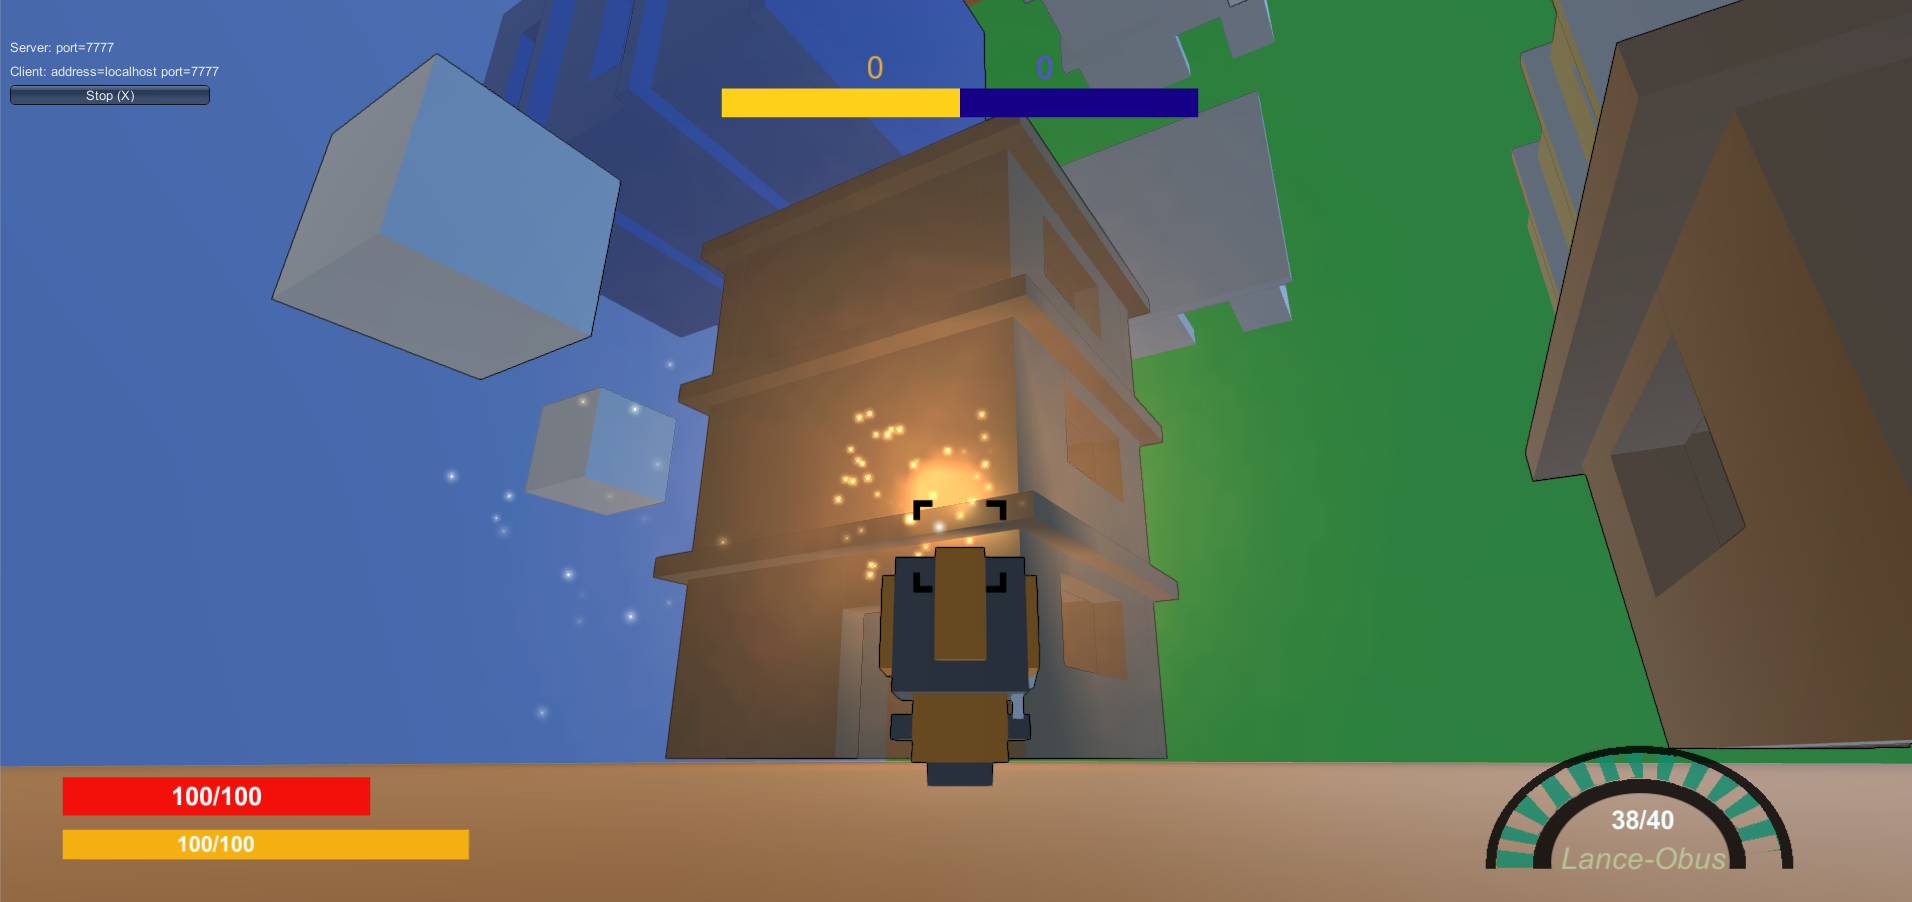
\includegraphics[scale=0.4]{explosion.png}}


\subsection {Physique}
La plus grosse partie de la physique était déjà disponible à la soutenance precedente, mais globalement,
celle-ci est plus fluide mais surtout, est présente sur certaines munition. Dans un soucis de réaelisme,
car oui marcher sur les murs est réaliste, une gravité est maintenant présente sur les obus et cette
gravité depend du joueur, sur quel mur il est aligné.


\subsection {Armes}
En plus d'une refonte graphique, toutes les armes ont subis une refonte au niveau du code. Ainsi elles sont
maintenant fonctionnelles en réseau. Le sniper, petit nouveau a cette soutenance dispose de son système de zoom,
qui changera le FoV de la caméra. Le lance flamme maintenant complet inflige correctement les dégâts.
Le lance grenade aussi, nouveau, s'ajoute au contenu du jeu. Les armes sont aussi maintenant dangereuses,
les joueurs prendrons des dégâts des différentes munitions mais aussi et surtout, certains parties des 
cartes seront aussi destructibles et prennent des dégâts des armes.


\subsection {Modèles}
Tout comme le site, les modèles ont fait peau neuve. Toutes les armes ainsi que le personnage sont dotés
de nouveaux modèles, en accord les un avec les autres. Cette partie fut particulièrement longue pour
respecter les critères graphiques du jeu, mais aussi pour que une sniper ressemble bien a un sniper, 
mais cubique.

\centerline{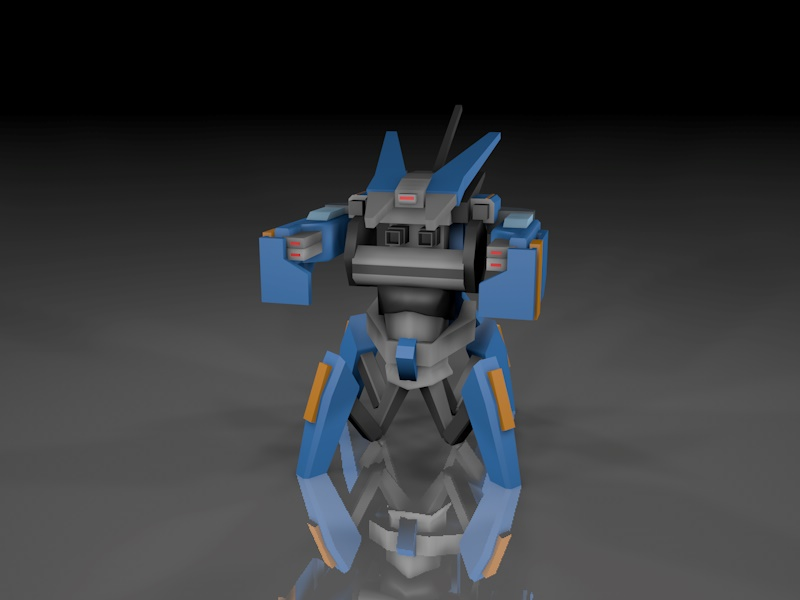
\includegraphics[scale=0.5]{NewPlayer.jpg}}
\subsection{Interface}
Menu pricipal:
\newline Nous avons finalement opté pour une charte graphique très simple basé sur le fait que les robots étant créer a partir de peu de moyen (le monde d'issidi étant détruit) toute les interfaces et même les retours fournis par le robot sont simplifier a l'extrême. Notre refonte de toutes les interfaces déjà existantes et la création des nouvelles se basent sur l'utilisation des canevas et non plus du GUI.
\newline\newline Menu principal:
\newline Ce menu permet de sélectionner les modes de jeu , et redirige vers les menus approprié.
\newline\newline  L'HUD:  
\newline L'interface de nos personnages est désormais composé de barres de vie et d'énergie qui fonctionne sont toute deux des images qui utilise la très pratique propriété "filled" qui gère automatiquement le remplissage en fonction du ratio. Nous avons aussi l'indispensable jauge de munition, un affichage des scores qui n'est pas encore synchronisé au niveau du serveur, et une crosshair pour visé.
\newline L'écran de mort
\newline Pour l'écran de mort nous avons choisit d'afficher le pseudo écran de l'utilisateur du drone. Ainsi il voit donc un écran bleu lui permettant soit de créer un nouveau robot soit de quitter complètement l'application.
\newline\newline Le menu de sélection multi:  
\newline Ce menu est très important il permet de choisir son équipe et son arme et ainsi d'enclencher le processus de création du personnage.
 
\subsection {IA}
L'IA de notre jeu est pour le moment rudimentaire mais celle-ci s'annonce plutôt intéressante.
Pour le moment seul deux ia sont développés et fonctionnels à leurs niveaux, la tourelle et la mine téléguidée.
La tourelle utilise un système de raycast en direction du joueur ainsi que d'une zone de détection afin de savoir
si celui-ci est perçu par la tourelle. Le point fort de cette méthode et que cela prend en compte la présence des
murs qui seraient entre la tourelle et le joueur. Si une détection est faite alors la tourelle se tourne vers le
joueur avec un délai de rotation permettant à celui-ci de se mettre à l'abri. Puis après un délai fixe la tourelle
se met à faire feu sur le joueur. Par la suite si le joueur sort de la zone de vision ou de détection de la tourelle
celle-ci arrête de tirer et se prépare de nouveau à le détecter.
La mine, elle, ne prend en compte que la distance réelle entre elle et la totalité des joueurs. Elle prend alors le
joueur le plus proche d'elle et en fait ça cible. Cependant si un autre joueur passe entre la mine et le joueur cible
il devient alors la nouvelle cible. Elle n'est pour le moment pas capable de différencier les joueurs des 2 équipes.
Une fois en collision elle détecte tous les joueurs dans une zone prédéfinie autour d'elle et leur inflige des dommages.
Si celle-ci n'atteint pas de cibles avant un certain temps elle s'autodétruit et fait de même que si elle avait touché une cible.
\subsection{Network}
\subsubsection {Adaptation des anciens scripts au reseau}
Les anciens scripts étant conçus pour fonctionner uniquement en singleplayer,
or lors de l'ajout du reseaux, un problème est apparu :
Si un personnage se déplaçait, en appuyant sur les touches directionnelles,
les autres joueurs se déplaçait aussi, ce qui n'est pas le comportement attendu.
Afin de pallier à ce problème, nous avons du dériver tous nos scripts non plus de
\begin{verbatim} MonoBehaviour \end{verbatim}, mais de \begin{verbatim} NetworkBehaviour \end{verbatim}
, qui propose une propriété interressante :
\begin{verbatim} isLocalPlayer \end{verbatim}.
Ainsi, cela nous permet de désactiver tous les scripts qui n'appartiennent pas au joueur local en faisant :
\begin{verbatim} enabled = isLocalPlayer \end{verbatim}
Cela à du être fait sur tous les anciens scripts, afin qu'ils fonctionnent en multijoueur.

\subsubsection {Interpolation}
Un problème que pose aussi le reseau, est le problème de lag (ou retard) qui peut arriver à tout moment dans une partie.
Afin de ne pas voir les déplacement saccadés des autres joueur, nous avons créer un script d'interpolation, qui s'attache
non pas uniquement au joueur, mais à toutes les entités dont nous voulons qu'elle apparaissent fluide en jeu (ce script fonctionne
donc aussi sur les balles que tirent les personnages).
Pour cela, nous avons utiliser la propriété \begin{verbatim} hadAuthority\end{verbatim}, et avons synchronisé la vitesse du
\begin{verbatim} RigidBody \end{verbatim} ainsi que sa rotation. Nous avons choisi de synchroniser la vitesse au lieu de la
position, afin de non plus ratrapper le "retard" a chaque frame, mais de pouvoir aussi prédire où le joueur vas aller,
pour avoir une sensation en multijoueur d'un jeu plus réactif.

\subsubsection {Tir du joueur}
Un fonctionnalité importante en multijoueur est le tir (principalement sur les enemis).
Pour avoir des tirs de balles fonctionnelles, nous avons dû, en plus de faire
\begin{verbatim} Instantiate(bullet) \end{verbatim} où \begin{verbatim} bullet \end{verbatim}
est un préfabriqué de la balle à faire apparaître lors du tir, faire apparaître les balles
sur le serveur, grâce à la commande suivante :
\begin{verbatim}
[Command]
void Cmd_InstantiateBullet(Vector3 position, Quaternion rotation, Vector3 up)
{
    GameObject bullet = (GameObject)Instantiate(bullet_template, position, rotation);
    if (!bullet)
        return;

    NetworkServer.Spawn(bullet);
}
\end{verbatim}
L'ajout de \begin{verbatim} [Command] \end{verbatim} avant la fonction à pour but de dire que cette fonction doit être appellé
par le serveur, et \begin{verbatim} NetworkServer.Spawn(bullet); \end{verbatim} permet la création de la balles sur tous
les clients connectés à la partie, au contraire de l'ancien système qui ne permettait l'apparition de la balle que sur le client
ayant tiré celle-ci.

\subsubsection {Création des personnages}
Le fait de pouvoir changer de personnage à chaque mort étant un élément indispensable pour notre jeu afin de lui apporter
plus de dynanisme, il a donc fallu avoir un système permettant ceci.
Au contraire de la création des balles qui se faisait sur le serveur et dont celui-ci en avait l'autorité, la création
des personnages doit se faire afin que le client voulu en ait l'autorité.
Pour ce faire, il a fallu faire une commande qui créé le personnage et l'assigne au joueur de cette manière :
\begin{verbatim}
[Command]
public void Cmd_CreatePlayer(Stats.Team team, int weapon_index)
{
    GameObject character = (GameObject)Instantiate(character_and_weapons[weapon_index]);
    //Tous les test d'erreurs on été enlevés pour montrer cet exemple
    NetworkServer.ReplacePlayerForConnection(connectionToClient, character, playerControllerId);
}
\end{verbatim}
Dans cet exemple, team représente l'équipe que veut rejoindre le joueur, et weapon-index l'index représentant
l'arme qu'il a choisit. character-and-weapons étant une liste de préfabriqué contenant à la fois le joueur, et l'arme associée.
Ensuite, a la fin de cette fonction, nous récupéront tous les \begin{verbatim} gameObject \end{verbatim} possédant le bon
tag de spawn (soit "WhiteSpawn" pour les spectateur, "OrangeSpawn" et "BlueSpawn"), et choisissont aléatoirement un des spawns,
afin de placer le joueur sur celui-ci, grâce à :
\begin{verbatim}
spawns[Random.Range(0, spawns.Length)].GetComponent<Spawner>().Spawn(character);
//Encore une fois, tous les test d'erreurs on été enlevés pour plus de claireté.
\end{verbatim}

\subsection {Autres}
\subsubsection {ColorModifier}
\begin{verbatim} {ColorModifier} \end{verbatim} est un script très utile dans notre jeu : en fonction de l'équipe dans lequel
le joueur est, il le colorie de la bonne façon, en récupérant tous les matériaux et en changeant les bons, de la façon suivante :
\begin{verbatim}
foreach (Transform child in transform)
{
    Material mat = child.gameObject.GetComponent<Renderer>().material;
    if (NeedChange(mat.color))
        mat.color = to_apply.color;
}
\end{verbatim}
De plus, ce script a été conçus de façon a pouvoir être attaché à n'importe quel objet.
Ainsi, cela nous permet de ne concevoir qu'un seul modèle, et de changer sa couleur, au lieu de
devoir avoir un modèle pour chaque équipe. Cela nous permet donc de simplifier la création des
personnages, ainsi que de leur gestion.

\subsubsection {Stats}
Ce script est un élément important du personnage : c'est lui qui gère la vie, l'énergie, les munitions du personnage.
Ainsi, la plupart des scripts se réfère à lui pour savoir si le personnage peut tirer, dasher, ou tout simplement si 
le personnage est mort.

\subsubsection{Site web}
	Avancement:
	A ce jour le site web est toujours en ligne à l'adresse : Issidi.shost.ca.
    Depuis la première soutenance le site web a subit une refonte complète dans le but de le rendre bien plus agréable a l'œil que sa précédente version. On peut bien entendu toujours avoir rapidement acces a toute nos ressources.
\subsubsection {Camera}
La caméra a été retravaillée pour cette soutenance, afin de ne plus passer à travers les murs.
Pour ce faire, nous récupéront l'axe sur laquelle la caméra doit se déplacer, et lançont un Raycast afin de voir
la présence d'un mur. Si il y en a un, nous modifions la position de la caméra afin de placer celle-ci juste avant le mur.

\subsubsection {Son}
L'ajout du son lors des mouvements du personnage permet de donner une meilleure immersion dans le jeu.
Afin d'ajouter cette partie imporante, nous avons créer une liste de sons de pas, prenons un son dans cette liste et le jouons
losrque le joueur marche. Lorsque le son s'arrete mais le le joueur est toujours sensé marcher, nous prenons alors le son suivant
et répétons cette procédure. Ainsi, le code à alors cette forme :
\begin {verbatim}
void Update ()
{
    if (!audio_source.isPlaying && deplacement.IsWalking())
    {//La gestion des erreurs a été enlevé pour plus de claireté
        audio_source.clip = footstep_sound[actual_sound];
        audio_source.Play();

        //Loop to next sound
        actual_sound = (actual_sound + 1) % footstep_sound.Count;
    }
}
\end{verbatim}
	
\section{Planning de la 3\ieme{} soutenance}
\begin{tabular}{|c|c|}
\hline
			& Troisième soutenance\\ \hline
Site Web	& XXX	\\ \hline
Physique	& XXX	\\ \hline
Multijoueur	& XXX	\\ \hline
Animation	& XXX	\\ \hline
IA	        & XXX	\\ \hline
Particules	& XXXX	\\ \hline
Personnage	& XXX	\\ \hline
Arme		& XXX	\\ \hline
Son			& XXX	\\ \hline
Modèles		& XXX	\\ \hline
interface	& XXX	\\ \hline
\end{tabular}

\section{Récit de la réalisation}
\subsection{Issidi.shost.ca}
Toujours confronté a l'éternel problème de la page blanche même si celle ci est resté virtuelle, nous avons tout de même en s'inspirant d'autre site réussi a obtenir un meilleur résultat que la première fois d'un point de vue visuel.
 

\subsection*{Interface}
La réalisation de l'interface ne fut pas une tâche aussi aisé qu'elle n'aurait pu l'être pour une raison simple. Lors des première réalisation la volonté de réellement "coder" quelque chose nous avait conduit a se tourner dans un premier temps vers le GUI qui est supposé être plutôt utilisé pour le debug, et n'aurait de toute façon pas été adapté pour l'implémentation du mode multijoueur par la suite.Nous nous sommes tout de même forcé a faire de L'UI qui, une fois qu'on arrête d'essayer de tout gérer par le code , se révèle plutôt efficace.

\subsection{animation}
La réalisation des animations nous a amené a nous confronter a blender logiciel que nous ne maîtrisions pas du tout. Et même si nous avons trouver de nombreux tutoriel qui expliquait comment faire. La présence de très nombreux nombreux raccourcis clavier pour changer l'angle de vue ou encore pour ouvrir les différents menus nous a beaucoup  ralentit. D autre petite subtilité comme par exemple le fait de ne pas pouvoir rouvrir un fichier .fbx enregistrer par blender avec ce dernier.Nous ont bien ralentit, néanmoins nous commençons maintenant nous y habitué.

\subsection {IA}

L'IA a été très intéressante pour le moment à faire car il y a toujours un problème ou un cas auquel on 
n'a pas pensé qui ce produit. En effet lors du codage du script de la tourelle celle-ci faisait tout sauf 
ce que l'on lui demandait.
En effet celle-ci se mettait à tourner sur elle-même sans jamais se fixer dès qu'un joueur était détecté. 
Quand celle-ci bougeait le référentiel n'était pas fixé et les coordonnées étant fixe la tourelle essayaient 
de rejoindre un point qu'elle ne pouvait rejoindre.

\subsection {Map}
Lors de la création de la map un problème est vite apparu : le trop grand nombre de setpasscall. En effet ceci est lié au nombre d'appel aux textures qui ont lieu sur la map.
Le problème et que plus celui-ci est élevé plus le nombre d'image par seconde chute et moins le jeu est jouable. Le but était donc de réduire celui-ci au maximum.
Le problème est que cela est très difficile de diminuer le nombre de setpasscall car nous essayons d'avoir un nombre d'entités suffisant pour que le décor soit destructible.
De plus même si une texture est réutilisée, de nouveaux setpasscalls apparaissent. Par la suite nous n'avons pas réussi à faire une carte véritablement destructible car générant trop d'objet et donc de setpasscall.
Notre carte solo ne sera donc un peu moins optimisé que celle en ligne pour le moment car celle-ci n'utilise pas beaucoup d'objet.

\subsection {Réseaux}
Unity est une formidable source de peines à propos du réseaux, où chaque mot de la documentation  d'Unity est très important. AInsi, la création du reseaux était un moment de tendre douleur, où ce qui marchait en mode un joueur, n,e marchait pas en mode multi. Une lecture attentive de toute la documentation est donc obligatoire.

\section{Conclusion}
Dans l'ensemble nous sommes très contents de ce qu'on a fait jusque la avec un gameplay très dynamique. le jeu marche en multi et est très fun , certaine personnes extérieur qui y ont joué se sont amusé aussi. Ces retours positif nous encourage donc a persévérer pour finir le jeu d'ici la dernière soutenance.
\end{document}

